%% LaTeX2e class for seminar theses
%% sections/content.tex
%% 
%% Karlsruhe Institute of Technology
%% Institute for Program Structures and Data Organization
%% Chair for Software Design and Quality (SDQ)
%%
%% Dr.-Ing. Erik Burger
%% burger@kit.edu
%%
%% Version 1.0, 2018-04-16


\section{Anforderungen}
\label{anfo}
Wie bereits in Kapitel \ref{projektrahmen} geschildert, soll der Adapater im Projekt Trust 4.0 eingesetzt werden. Daraus egeben sich einige Anforderungen, damit eine Integration in die bestehende Codebasis m"oglich ist.\newline
Der Adapter soll in dem projekteignen Eclipse-Plugin eingesetzt werden. Dieses Plugin ist unter der Eclipse Plugin Licence (EPL)\cite{epl} lizenziert, was zu der Anfordung f"uhrt, dass Software, die in dem Plugin zum Einstaz kommt, auch unter EPL oder zu EPL kompatibel lizenziert sein muss. Diese Anforderung gilt ebenso f"ur den Adapter und die durch ihn angebundene Interpreter.\newline
SWI-Prolog\cite{swi} ist der quasi Standard-Interpreter in der Prologwelt. Kein anderer Interpreter ist in dem Ma"se verbreitet und wird auch dementsprchend aktiv weiterentwickelt, weshalb eine Anbindung daran unerl"asslich ist. Au"serdem muss mindestens ein Weiterer der angebundenen Interpreter in Java implementiert sein. Der Grund daf"ur ist, dass das Plugin bei der Auslieferung m"oglichst wenige Abh"angigkeiten auf bereits vorinstallierte Software haben soll. Ein in Java implementierter Interpreter kann in das Plugin-Packet miteingebunden werden, wodurch der Nutzer nicht auf einen vorinstallierten Interpreter auf seinem System angewiesen ist. Im Nachhineinen gibt es jedoch immernoch die M"oglichkeit bei Bedarf auf SWI-Prolog o."a. zu wechseln.\newline
Wenn man Anfragen an einen Interpreter im interaktiven Modus im Terminal schickt, "ubergibt man die Anfrage selbst als einen String und als Antwort erh"alt man ebenfalls einen String. Dieses Verhalten ist gew"unscht, wenn man in einem Terminal arbeitet, da man die Ergebnisse in der Regel nicht programmatisch weiterverarbeiten will. Sendet man Anfragen jedoch, wie in unserem Fall, aus Java-Code heraus, will man mit dem Ergebnis einer Anfrage weiter arbeiten. Da w"are es unvorteilhaft, w"urde man als Antwort vom Interpreter ausschlie"slich Strings erhalten, da man diese erst selbst in ein gew"unschte Format parsen m"usste. Solche Parser sind fehleranf"allig und aufw"andig zu implementieren, bringen aber gleichzeitig dem Projekt wenig Mehrwert. Deshalb sollten
man bei der Verwendung des Adpaters bereits verwertebare Objekte als Antwort erhalten, wie beispielsweise \emph{Integer}, \emph{Float} oder selbst definierte Klassen.

\section{Interpreterwahl}
In Kapitel \ref{anfo} wurde bereits SWI-Prolog als ein anzubindenden Interpreter fest vorgebeben, sowie die beiden Anforderungen, dass die Interpreter EPL-kompatibel lizenziert sein m"ussen und au"serdem mindestens ein Interpreter in Java implementiert sein muss. \newline
Insgesamt habe ich die Wahl, welche Interpreter angebunden werden sollen, nach folgenden Kriterien getroffen: \textbf{(* Pflicht)}\newline
\newline
\textbf{EPL-kompatibel lizenziert*} Der Adapter wird Teil eines Eclipse-Plugins sein, welches unter EPL lizenziert ist. Daraus ergibt sich, dass ein verwendeter Interpreter mit EPL kompatibel lizensiert sein muss.\newline
\textbf{Java-Schnittstelle*} Um einen Interpreter von Java-Code aus zu verwenden muss dieser bereits eine eigene Java-Schnittstelle mitbringen. Es w"are zwar m"oglich auch selber eine solche Schnittstelle zu entwickeln, allerdings liegt das au"serhalb des Umfangs dieses Praktikums.\newline
\textbf{Paket im Maven-Repository} Ein Paket, welches im Maven-Repository liegt, kann ohne gro"sen Aufwand in den Build-Prozess eines Projektes eingebunden werden. Dies verringert den Wartungsaufwand und stabilisiert den Build-Prozess "uber Platformen und Ger"ate hinweg, da ein Paket direkt aus dem Repository geladen werden kann, anstatt dass nach lokalen Bibliotheken gesucht werden muss. Ein Interpreter, der seine Java-Schnittstelle als Packet im Maven-Repository bereitstellt, verursacht daher allgemein weniger Aufwand bei der Einbindung.\newline
\textbf{Java-Implementierung} Mindestens ein Interpreter sollte in Java implementiert sein, sodass dieser mit dem Plugin zusammen ausgeliefert werden kann. Dadurch muss der Nutzer keinen eigenen Interpreter auf seinem System installieren.\newline
\textbf{Zeitpunkt des letzten Releases} Ein Projekt, welches nicht gewartet wird, bringt ein gewisses Risiko bei der Verwendung mit sich. Zum Einen werden logische Programmfeheler, die zu falschen Ergebnissen bei Berechnungen f"uhren k"onnen, nicht mehr gefixt und zum Anderen k"onen auch ungepatchte Sicherheitsl"ucken zu einem Problem f"ur den Nutzer werden. Au"serdem kann mit der Ver"offentlichung neuer Versionen von Drittsoftware die Kompatibilit"at mit veralteten Projekten gebrochen werden. Daher ist es wichtig, dass ein Interpreter, zumindest zum jetzigen Zeitpunkt, noch aktiv weiter entwickelt wird.\newline
\newline
Da eine EPL-kompatible Lizenz und eine bereits vorhandene Java-Schnittstelle Pflichtkriterien sind, werde ich in der folgenden Vorstellung der ausgew"ahlten Interpreter nur in besonderen F"allen weiter darauf eingehen.
\subsection{SWI-Prolog}
SWI-Prolog\cite{swi} ist der am weitestverbreiteste und am aktivsten weiter entwickelte Interpreter. Deswegen wurde in Kapitel \ref{anfo} bereits vorrausgesetzt, dass dieser Interpreter angebunden werden sollte. Neue Versionen werden teilweise im Wochentakt ver"offentlicht, weshalb eine Veraltung des Projektes in n"achster Zeit nicht zu erwarten ist. Au"serdem stellt SWI-Prolog eine Maven-Paket zur Verf"ugung, welches allerdings eine Abh"angigkeit auf eine native Bibliothek hat. Dies setzt vorraus, das der Nutzer bereits SWI-Prolog installiert und sein System so konfiguriert hat, dass die JVM in der Lage ist, diese Bibliothek auch zu finden.
\subsubsection{Installation unter Linux}
\textbf{Zu installierende Pakete}: swi-prolog-devel\newline
\newline
Nachdem dieses Paket installiert wurde, sollte das Verzeichnis \emph{/usr/lib/swipl/lib/} existieren. Je nach Architektur liegt in diesem Verzeichnis ein Ordner \emph{x86-linux} oder \emph{x86\_64-linux}, worin wiederum eine Datei \emph{libjpl.so} liegt. F"uhren Sie folgenden Befehl im Terminal aus: (Beispiel 64-bit Architektur)\newline
\begin{minted}{bash}
ln -s /usr/lib/swipl/lib/x86_64-linux/libjpl.so /usr/lib/.
\end{minted}
Dieser Befehl erstellt eine Verkn"upfung der Datei \emph{libjpl.so} im Verzeichnis \emph{/usr/lib/libjpl.so}.

\subsection{TuProlog}
TuProlog\cite{tuprolog} ist ein in Java implementierter Interpreter. Er verfolgt die Philosophie, einen m"oglichst kleinen Kern zu haben und zus"atzliche Funktionalit"aten "uber Bibliotheken nachzuladen. Lizenziert ist er unter LGPL, welche im Allgemeinen nicht EPL-kompatibel ist\cite{eplkompatibel}. Jedoch wurde diese Lizenz in der Vergangenheit in einzelnen F"allen doch als kompatibel anerkannt, weshalb es hier eine gewisse Grauzone zu geben scheint. Au"serdem befindet sich das Projekt Trust 4.0 momentan noch im Bereich des 'non commercial use', weshalb die Nutzung dieses Interpreter vorerst ohnehin keine Schwierigkeit darstellt. Der letzte Release von TuProlog war im Juli 2019, allerdings nutzte ich in meinem Adapter noch die Version vom Oktober 2018, da ich mit der Implementierung bereits im Juni begonnen hatte. TuProlog ist au"serdem als Paket im Maven-Repository verf"ugbar, weshalb von Nutzerseite aus keine weitere Installation erforderlich ist.

\subsection{Projog}
Projog\cite{projog} ist ebenfalls ein in Java implementierter Interpreter. Im Gegensatz zu den beiden anderen Interpretern ist dieses Projekt noch sehr jung, wird aber dementsprechend auch noch weiter entwickelt. Ein Nachteil dieser Implementierung ist allerdings, dass sie noch nicht ganz konform zum Prolog ISO Standard ist, weshalb durchaus an einigen Stellen die Funktionalit"at eingeschr"ankt sein k"onnte. Projog steht, wie TuProlog, als Paket im Maven-Repository zur Verf"ugung und kann somit automatisch durch Maven eingerichtet werden und erfordert keine Installation oder Konfigration nutzerseitens.

\section{Prolog4J}
Prolog4J\cite{prolog4j} ist eine bereits existierende Bibliothek, die verschiedene Prolog Interpreter an Java anbindet. Da der Code unter der MIT Lizenz steht, also EPL-kompatibel ist, kann ich darauf aufbauen und den Adapter so anpassen, dass er den in Kapitel \ref{anfo} geschilderten Anforderungen gerecht wird. Au"serdem ist Prolog3J relativ gut dokumentiert\cite{prolog4jdoku}.

\subsection{Architektur}
Prolog4J setzt auf einen minimalistischen Ansatzt. Der Kern der Bibliothek ist relativ klein und besteht lediglich aus 14 Klassen. In Abbildung \ref{fig:prolog4jj} ist ein grobes Klassendiagramm des Adapater dargestellt.
\begin{figure}[h]
\centering
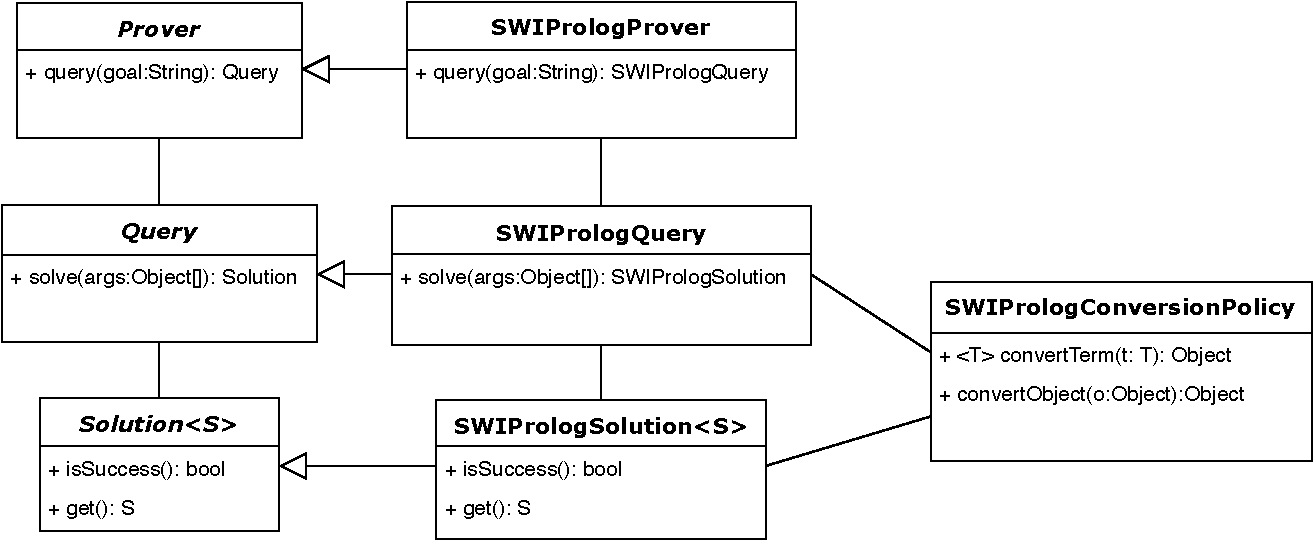
\includegraphics[width=0.9\textwidth]{prolog4j.pdf}
\caption{Die API besteht aus Prover, Query und Solution, die jeweils f"ur einen konkreten Interpreter spezialisiert werden.}
\label{fig:prolog4jj}
\end{figure}


\subsection{Anpassungen}
Prolog4J bietet nicht alles was ben"otigt ist und bringt auch inige Probleme mit sich. Von selbst unterst"utzt es die Interpreter SWI, TuProlog, JTrolog und JLog, allerdings nicht Projog. Das hei"st zum einen m"ussen die "uberfl"ussigen Interpretr entfernt und Projog noch hinzugef"ugt werden. Des weiteren wurde das Projekt seit 2011 nicht mehr weiter entwicketlt, das hei"st dass zum einen die Maven Build dateien gupdatet werden m"ussen, also Paket-Versionen m"ussen angepasst werden, und ver"anderungen in den APIs in den POM m"ussen auch ber"ucksichtig werden. Au"serdem muss noch der Code aktualisiert werden. Denn die Schnittstellen der Interpretr wurden in der Zwischenzeit auch weiterentwickelt. Als letztes muss ich nich fehlende Funktionalit"at hinzuf"ugen. Zum einen m"ussen Fakten aus einer Datei gelesen werden, eine Interpretrinstanz muss zur"uckgestzt werden k"onnen und es muss OSGI discovery funktionieren.

\subsection{Besonderheiten}
In diesem Kapitel werde ich einige Besonderheiten erkl"aren, die mir bei der Implementierung aufgefallen sind.

\subsubsection{Bug in Projog}
Ein Fakt ist ein Ausdruck der Form name(inhalt). Diese Fakten werden in einer Datenbank gespeichert und k"onnen durch Abfragen abgrfragt werden. Projog speichert diese Fakten in einer Hashmap und verwendet dabei den Faktennamen als Key. F"ugt man nun ein Fakt der Datenbank hinzu wird der Name als Key. Beispiel Hashmap zeigen./ W"urde man weitere Fakten hinzuf"ugen, s"ahe die Hashmap so aus. Projog allerdings f"ugt neue Fakten nicht den alten hinzu, sondern ersetzt die bestehenden Fakten. Das ist kein Problem, wenn die Datenbank leer ist, und man alle ben"otigten Fakten auf einmal HinzuF'ugt. Projog erstellt eine Liste an Fakten und F'ugt sie dann der HashMap hinzu. Problemnatisch wird es, wenn man Fakten einzeln hinzuF'ugt. Beispiel erkl"aren. Um dieses Problem zu l"osen halte ich eine eigne HashMap und F'uge neue Fakten erst dort ein und danach die gesamten Werte in die Projog Datenbank.
\subsubsection{Cons-Operator in SWI-Prolog}

\subsubsection{Paramtererstezung in SWI-Prolog Termen}


\subsection{OSGI}














